\documentclass{../vespers-booklet}
\usepackage{multicol}

\begin{document}

\chapter*{First Vespers of the Transfiguration of Our Lord Jesus Christ}

\vspace{0.5mm}

\begin{center}
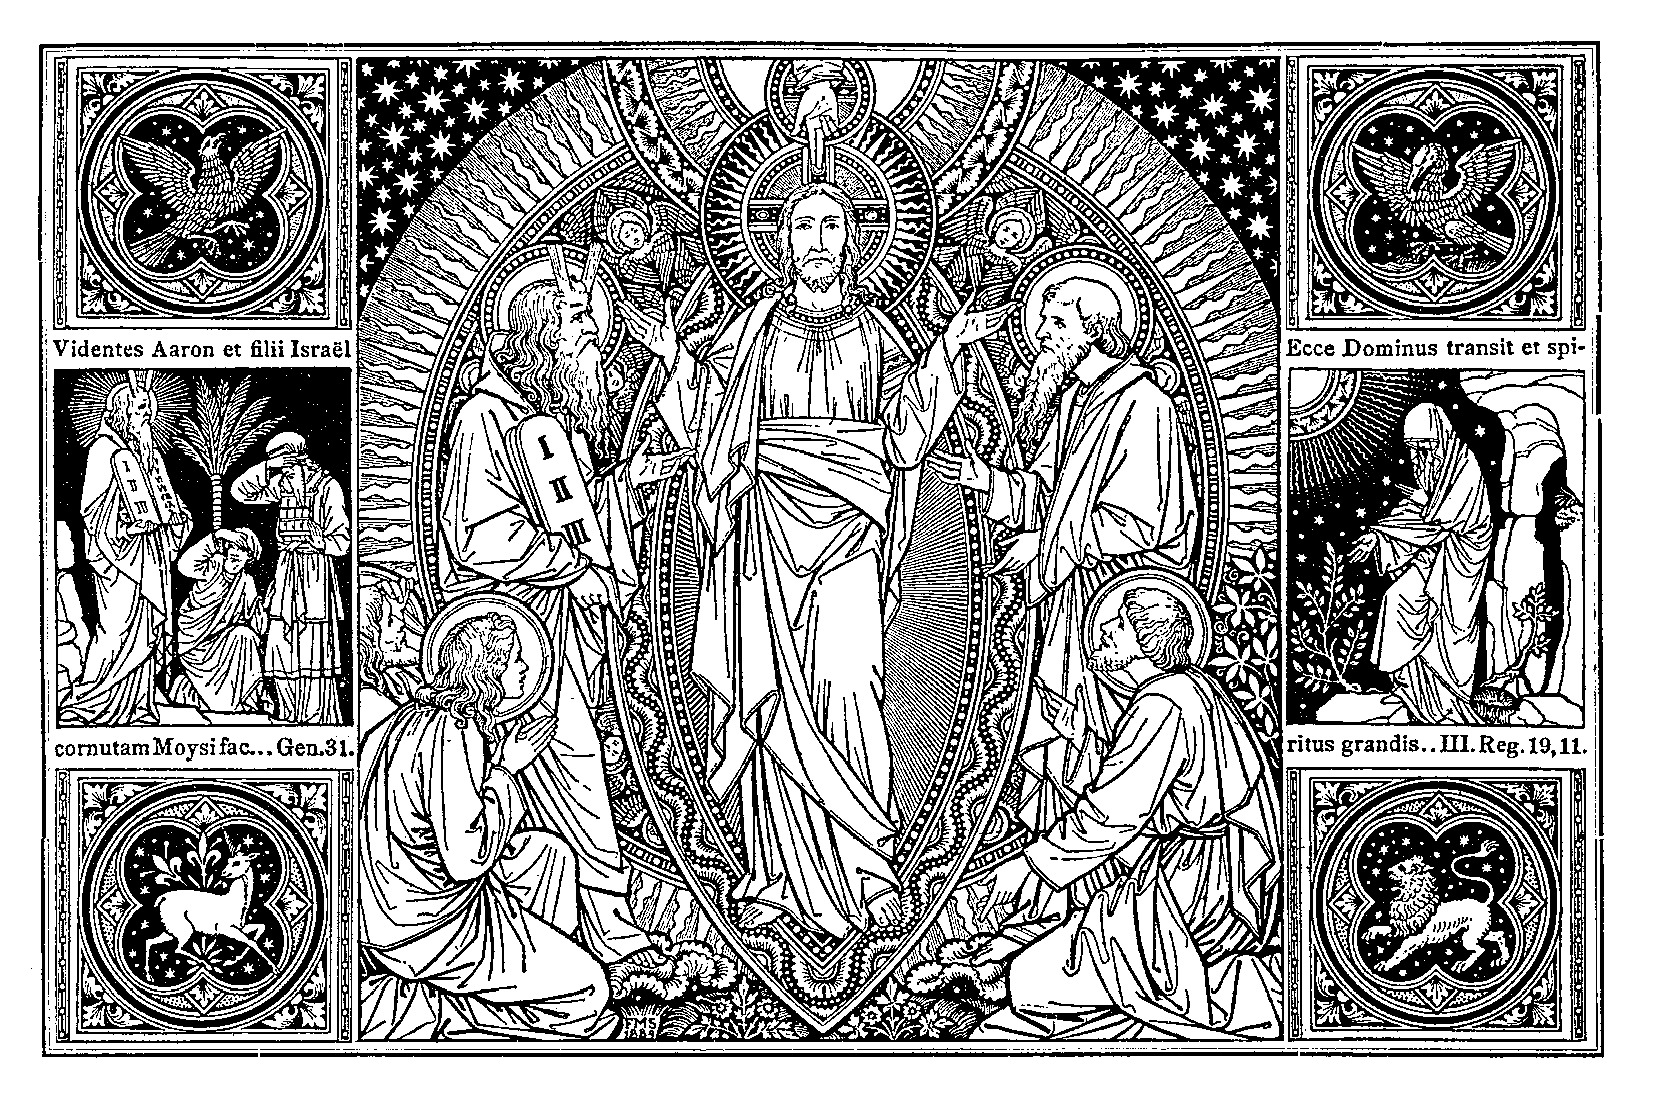
\includegraphics[width=\textwidth]{Transfiguration.jpg}
\end{center}

\vfill\pagebreak

\begin{rubricbox}

{\color{red}When the Officiant kneels, all \textbf{kneel} and pray silently.
Then, when the Officiant stands, all \textbf{stand} and say silently one \textit{Pater noster} (Our Father) and \textit{Ave Maria} (Hail Mary).
Then all make the sign of the cross with the Officiant as he intones:}

\end{rubricbox}

\gresetinitiallines{1}
\gregorioscore{../common/deus-in-adjutorium-solemn}

\textit{
O God, come to my assistance.
{\color{red}\Vbar.}~O Lord, make haste to help me.
Glory be to the Father, and to the Son, and to the Holy Spirit,
as it was in the beginning, is now, and ever shall be, world without end. Amen.
Praise to Thee, O Lord, King of endless glory.}

\vfill\pagebreak

%% FIRST PSALM

\section*{Psalm 109}

\textit{\textnormal{Ant. 1.} Jesus took Peter, * and James, and John his brother, and brought them up into an high mountain apart and was transfigured before them.
 \textnormal{Ps.} The Lord said to my Lord: * Sit thou at my right hand:}
 
 \begin{rubricbox}

{\color{red}All remain standing throughout the first antiphon.
After the psalm is intoned by the Cantor, all \textbf{sit} at the asterisk. This is done for the remaining Psalms.}

\end{rubricbox}

\gresetinitiallines{1}
\gregorioscore{ps109-antiphon}

\gresetinitiallines{0}
\gregorioscore{ps109-intonation}

 \begin{latinenglishsection}

\latinenglish{

	2. Donec ponam ini\textbf{mí}cos \textbf{tu}os,~*
	scabéllum pe\textit{dum} \textit{tu}\textbf{ó}rum.

3. Virgam virtútis tuæ emíttet Dómi\textbf{nus} ex \textbf{Si}on:~*
	domináre in médio inimicó\textit{rum} \textit{tu}\textbf{ó}rum.

4. Tecum princípium in die virtútis tuæ in splendóri\textbf{bus} sanc\textbf{tó}rum:~*
	ex útero ante lucíferum \textit{gé}\textit{nu}\textbf{i} te.

5. Jurávit Dóminus, et non p{\oe}ni\textbf{té}\-bit \textbf{e}um:~*
	Tu es sacérdos in ætérnum secúndum órdi\textit{nem} \textit{Mel}\textbf{chí}se\-dech.

6. Dóminus a \textbf{dex}tris \textbf{tu}is,~*
	confrégit in die iræ \textit{su}\textit{æ} \textbf{re}ges.

7. Judicábit in natiónibus, im\textbf{plé}bit ru\textbf{í}nas:~*
	conquassábit cápita in ter\textit{ra} \textit{mul}\textbf{tó}rum.

8. De torrénte in \textbf{vi}a \textbf{bi}bet:~*
	proptérea exal\textit{tá}\textit{bit} \textbf{ca}put.

9. \textit{(bow)} Glória \textbf{Pa}tri, et \textbf{Fí}lio,~*
	et Spirí\textit{tu}\textit{i} \textbf{Sanc}to.

10. \textit{(rise)} Sicut erat in princípio, et \textbf{nunc}, et \textbf{sem}per,~*
	et in s\'{\ae}cula sæcu\textit{ló}\textit{rum}. \textbf{A}men. %%

}{
	% 1. The Lord said to my Lord: Sit thou at my right hand:

2. Until I make thy enemies thy footstool.
 
3. The Lord will send forth the sceptre of thy power out of Sion: rule thou in the midst of thy enemies.
 
4. With thee is the principality in the day of thy strength: in the brightness of the saints:
 from the womb before the day star I begot thee.
 
5. The Lord hath sworn, and he will not repent: Thou art a priest for ever according to the order of Melchisedech.
 
6. The Lord at thy right hand hath broken kings in the day of his wrath.

7. He shall judge among nations, he shall fill ruins: he shall crush the heads in the land of the many.

8. He shall drink of the torrent in the way: therefore shall he lift up the head. 

Glory be. %%
}

\end{latinenglishsection}

\gresetinitiallines{1}
\gregorioscore{ps109-antiphon}

%\begin{rubricbox}

%{\color{red} The antiphon is repeated: \textit{Assúmpsit Jesus\dots}} %%

%\end{rubricbox}

\vfill\pagebreak

%% SECOND PSALM

\section*{Psalm 110}

\textit{\textnormal{Ant. 2.} His Face did shine as the sun, * and His raiment exceeding white as snow, alleluia.
 \textnormal{Ps.} I will praise thee, O Lord, with my whole heart; * in the council of the just, and in the congregation.}

\gresetinitiallines{1}
\gregorioscore{ps110-antiphon}

\gresetinitiallines{0}
\gregorioscore{ps110-intonation}

 \begin{latinenglishsection}

\latinenglish{

	2. Magna ópera \textbf{Dó}mini:~*
	exquisíta in omnes volun\textit{tá}\textit{tes} \textbf{e}jus.

3. Conféssio et magnificéntia opus \textbf{e}jus:~*
	et justítia ejus manet in s\'{\ae}\textit{cu}\-\textit{lum} \textbf{s\'{\ae}}culi.

4. Memóriam fecit mirabílium suórum,~{\color{red}\GreDagger}\
	miséricors et miserátor \textbf{Dó}\-minus:~*
	escam dedit ti\textit{mén}\textit{ti}\textbf{bus} se.

5. Memor erit in s\'{\ae}culum testaménti \textbf{su}i:~*
	virtútem óperum suórum annuntiábit pó\textit{pu}\textit{lo} \textbf{su}o:

6. Ut det illis hereditátem \textbf{gén}ti\-um:~*
	ópera mánuum ejus véritas, \textit{et} \textit{ju}\textbf{dí}\-cium.

7. Fidélia ómnia mandáta ejus:~{\color{red}\GreDagger}\
	confirmáta in s\'{\ae}culum \textbf{s\'{\ae}}culi,~*
	facta in veritáte et \textit{æ}\textit{qui}\textbf{tá}te.

8. Redemptiónem misit pópulo \textbf{su}o:~*
	mandávit in ætérnum\\ testa\textit{mén}\textit{tum} \textbf{su}um.

9. Sanctum, et terríbile nomen \textbf{e}jus:~*
	inítium sapiéntiæ \textit{ti}\textit{mor} \textbf{Dó}\-mini.

10. Intelléctus bonus ómnibus faciéntibus \textbf{e}um:~*
	laudátio ejus manet in s\'{\ae}\textit{cu}\textit{lum} \textbf{s\'{\ae}}culi.

{\color{red}\textit{(bow)}} Glória Patri, et \textbf{Fí}lio,~*
	et Spirí\textit{tu}\textit{i} \textbf{Sanc}to.

{\color{red}\textit{(rise)}} Sicut erat in princípio, et nunc, et \textbf{sem}per,~*
	et in s\'{\ae}cula sæcu\textit{ló}\textit{rum}. \textbf{A}men. %%

}{
	 1. I will praise thee, O Lord, with my whole heart; in the council of the just: and in the congregation.
 
 2. Great are the works of the Lord: sought out according to all his wills.
 
 3. His work is praise and magnificence: and his justice continueth for ever and ever.
 
 4.  He hath made a remembrance of his wonderful works, being a merciful and gracious Lord: he hath given food to them that fear him. 	
 
 5. He will be mindful for ever of his covenant: he will shew forth to his people the power of his works.
 
 6. That he may give them the inheritance of the Gentiles: the works of his hands are truth and judgment.
 
 7. All his commandments are faithful: confirmed for ever and ever, made in truth and equity.
 
 8. He hath sent redemption to his people: he hath commanded his covenant for ever.
 
 9. Holy and terrible is his name: the fear of the Lord is the beginning of wisdom.
 
 10. A good understanding to all that do it: his praise continueth for ever and ever.  %%
}

\end{latinenglishsection}

\gresetinitiallines{1}
\gregorioscore{ps110-antiphon}

%\begin{rubricbox}

%{\color{red}The antiphon is repeated: \textit{Resplénduit\dots}} %%

%\end{rubricbox}

\vfill\pagebreak

%% THIRD PSALM

\section*{Psalm 111}

\textit{\textnormal{Ant. 3.} And, behold, there appeared unto them Moses and Elias, * talking with Jesus.
 \textnormal{Ps.} Blessed is the man that feareth the Lord: * he shall delight exceedingly in his commandments.}

\gresetinitiallines{1}
\gregorioscore{ps111-antiphon}

\gresetinitiallines{0}
\gregorioscore{ps111-intonation}

 \begin{latinenglishsection}

\latinenglish{

	2. Potens in terra erit \textit{se}\textit{men} \textbf{e}jus:~* generátio rectórum \textit{be}\textit{ne}\textit{di}\textbf{cé}tur.

3. Glória, et divítiæ in \textit{do}\textit{mo} \textbf{e}jus:~* et justítia ejus manet in \textit{s\'{\ae}}\textit{cu}\textit{lum} \textbf{s\'{\ae}}culi.

4. Exórtum est in ténebris \textit{lu}\textit{men} \textbf{rec}tis:~* miséricors, et mise\textit{rá}\textit{tor}, \textit{et} \textbf{jus}tus.

5. Jucúndus homo qui miserétur et cómmodat,~\GreDagger\ dispónet sermónes suos \textit{in} \textit{ju}\textbf{dí}cio:~* quia in ætérnum \textit{non} \textit{com}\textit{mo}\textbf{vé}bitur.

6. In memória ætérna \textit{e}\textit{rit} \textbf{jus}tus:~* ab auditióne ma\textit{la} \textit{non} \textit{ti}\textbf{mé}bit.

7. Parátum cor ejus speráre in Dómino,~\GreDagger\ confirmátum \textit{est} \textit{cor} \textbf{e}jus:~* non commovébitur donec despíciat in\textit{i}\textit{mí}\textit{cos} \textbf{su}os.

8. Dispérsit, dedit paupéribus:~\GreDagger\ justítia ejus manet in s\'{\ae}\textit{cu}\textit{lum} \textbf{s\'{\ae}}culi,~* cornu ejus exaltá\textit{bi}\textit{tur} \textit{in} \textbf{gló}ria.

9. Peccátor vidébit, et irascétur,~\GreDagger\ déntibus suis fremet \textit{et} \textit{ta}\textbf{bé}scet:~* {\color{red}\textit{(stand)}} desidérium pecca\textit{tó}\textit{rum} \textit{per}\textbf{í}bit.

{\color{red}\textit{(bow)}} Glória Pa\textit{tri}, \textit{et} \textbf{Fí}lio,~* et Spi\textit{rí}\textit{tu}\textit{i} \textbf{Sanc}to.

{\color{red}\textit{(rise)}} Sicut erat in princípio, et \textit{nunc}, \textit{et} \textbf{sem}per,~* et in s\'{\ae}cula sæ\textit{cu}\textit{ló}\textit{rum}. \textbf{A}men. %%

}{
	1. Blessed is the man that feareth the Lord: he shall delight exceedingly in his commandments.

2. His seed shall be mighty upon earth: the generation of the righteous shall be blessed.

3. Glory and wealth shall be in his house: and his justice remaineth for ever and ever.

4. To the righteous a light is risen up in darkness: he is merciful, and compassionate and just.

5. Acceptable is the man that sheweth mercy and lendeth: he shall order his words with judgment:
because he shall not be moved for ever.

6. The just shall be in everlasting remembrance: he shall not fear the evil hearing.

7. His heart is ready to hope in the Lord: his heart is strengthened, he shall not be moved until he look over his enemies.

8. He hath distributed, he hath given to the poor: his justice remaineth for ever and ever: his horn shall be exalted in glory.

9. The wicked shall see, and shall be angry, he shall gnash with his teeth and pine away: the desire of the wicked shall perish.  %%
}

\end{latinenglishsection}

\gresetinitiallines{1}
\gregorioscore{ps111-antiphon}

%\begin{rubricbox}

%{\color{red}The antiphon is repeated: \textit{Et ecce\dots}, then all \textbf{stand}} %%

%\end{rubricbox}

\vfill\pagebreak

%% FOURTH PSALM

\section*{Psalm 112}

\textit{\textnormal{Ant. 4.} Then answered Peter, * and said unto Jesus: Lord, it is good for us to be here.
 \textnormal{Ps.} Praise the Lord, ye children: * praise ye the name of the Lord.}

\gresetinitiallines{1}
\gregorioscore{ps112-antiphon}

\gresetinitiallines{0}
\gregorioscore{ps112-intonation}

 \begin{latinenglishsection}

\latinenglish{

	2. Sit nomen Dómini \textbf{be}ne\textbf{díc}tum,~* ex hoc nunc, et us\textit{que} \textit{in} \textbf{s\'{\ae}}culum.

3. A solis ortu usque \textbf{ad} oc\textbf{cá}sum,~* laudábile \textit{no}\textit{men} \textbf{Dó}mini.

4. Excélsus super omnes \textbf{gen}tes \textbf{Dó}minus,~* et super cælos gló\textit{ri}\textit{a} \textbf{e}jus.

5. Quis sicut Dóminus, Deus noster, qui in \textbf{al}tis \textbf{há}bitat,~* et humília réspicit in cælo \textit{et} \textit{in} \textbf{ter}ra?

6. Súscitans a \textbf{ter}ra \textbf{ín}opem,~* et de stércore é\textit{ri}\textit{gens} \textbf{páu}perem:

7. Ut cóllocet eum \textbf{cum} prin\textbf{cí}pibus,~* cum princípibus pó\textit{pu}\textit{li} \textbf{su}i.

8. Qui habitáre facit stéri\textbf{lem} in \textbf{do}mo,~* matrem filió\textit{rum} \textit{læ}\textbf{tán}tem.

{\color{red}\textit{(bow)}} Glória \textbf{Pa}tri, et \textbf{Fí}lio,~* et Spirí\textit{tu}\textit{i} \textbf{Sanc}to.

{\color{red}\textit{(rise)}} Sicut erat in princípio, et \textbf{nunc}, et \textbf{sem}per,~* et in s\'{\ae}cula sæcu\textit{ló}\textit{rum}. \textbf{A}men. %%

}{
	%1. Praise the Lord, ye children: praise ye the name of the Lord.
 	
2. Blessed be the name of the Lord, from henceforth now and for ever.
 	
3. From the rising of the sun unto the going down of the same, the name of the Lord is worthy of praise.
 	
4. The Lord is high above all nations; and his glory above the heavens.
 	
5.Who is as the Lord our God, who dwelleth on high, and looketh down on the low things in heaven and in earth?
 	
6. Raising up the needy from the earth, and lifting up the poor out of the dunghill:
 	
7. That he may place him with princes, with the princes of his people.
 	
8. Who maketh a barren woman to dwell in a house, the joyful mother of children. 

Glory be. %%
}

\end{latinenglishsection}

\gresetinitiallines{1}
\gregorioscore{ps112-antiphon}

%\begin{rubricbox}

%{\color{red}The antiphon is repeated: \textit{Respóndens autem Petrus\dots}} %%

%\end{rubricbox}

\vfill\pagebreak

%% FIFTH PSALM

\section*{Psalm 116}

\textit{\textnormal{Ant. 5.} While he yet spake, * behold, a bright cloud overshadowed them.
 \textnormal{Ps.} Praise the Lord, all ye nations: * praise him, all ye people.}

\gresetinitiallines{1}
\gregorioscore{ps116-antiphon}

\gresetinitiallines{0}
\gregorioscore{ps116-intonation}

 \begin{latinenglishsection}

\latinenglish{

	2. Quóniam confirmáta est super nos miseri\textbf{cór}dia \textbf{e}jus:~* {\color{red}\textit{(stand)}} et véritas Dómini manet \textit{in} \textit{æ}\textbf{tér}num.

{\color{red}\textit{(bow)}} Glória \textbf{Pa}tri, et \textbf{Fí}lio,~* et Spirí\textit{tu}\textit{i} \textbf{Sanc}to.

{\color{red}\textit{(rise)}} Sicut erat in princípio, et \textbf{nunc}, et \textbf{sem}per,~* et in sǽcula sæcu\textit{ló}\textit{rum}. \textbf{A}men. %%

}{
	1. O praise the Lord, all ye nations: praise him, all ye people.

2. For his mercy is confirmed upon us: and the truth of the Lord remaineth for ever.  %%
}

\end{latinenglishsection}

\gresetinitiallines{1}
\gregorioscore{ps116-antiphon}

%\begin{rubricbox}

%{\color{red}The antiphon is repeated: \textit{Adhuc eo loquénte\dots}, then all \textbf{stand}}

%\end{rubricbox}

\section*{Little Chapter (Phil 3:20-21)}

\textit{\color{red}The Officiant leads the Little Chapter:}

\begin{latinenglishsection}

\latinenglish{
	Salvatórem exspectámus Dóminum nostrum Jesum Christum,{\color{red}\GreDagger}\
	qui\\ reformábit corpus humilitátis nostræ configurátum córpori claritátis suæ.
	{\color{red}\Rbar.}~Deo grátias.
}{
	We look for the Saviour, the Lord Jesus Christ, Who shall change our vile body, that it may be fashioned like unto His glorious Body.
	 {\color{red}\Rbar.}~Thanks be to God.
}

\end{latinenglishsection}

\section*{Hymn}

\textit{\color{red}The Cantor leads the hymn:}

\gresetinitiallines{1}
\gregorioscore{../hymns/quicumque-christum--solesmes}

{\itshape

	1. All ye who would the Christ descry,
	Lift up your eyes to him on high:
	There mortal gaze hath strength to see
	The token of his majesty.
	
	2. A wondrous sign we there behold,
	That knows not death nor groweth old,
	Sublime, most high, that cannot fade,
	That was ere earth and heaven were made.
	
	3. Here is the King the gentiles fear,
	The Jews' most mighty King is here
	Promised to Abraham of yore,
	And to his seed forevermore.
	
	4. 'Tis he the prophets' words foretold,
	And by their signs shown forth of old;
	The Father's witness hath ordained
	That we should hear with faith unfeigned.
	
	5. Jesu, to thee our praise we pay,
	To little ones revealed today,
	With Father and blest Spirit One
	Until the ages' course is done.
	Amen.
}

\textit{\color{red}The Cantor says the following before all reply afterwards:}

\gresetinitiallines{0}
\gabcsnippet{
(c3) <c><sp>V/</sp>.</c> Glo(h)ri(h)ó(h)sus(h) ap(h)pa(h)ru(h)í(h)sti(h) in(h) con(h)spéc(h)tu(h) Dó(h)mi(f)ni.(g'_/hvGF'E/fgf.) (::)
}

\gresetinitiallines{0}
\gabcsnippet{
(c3) <c><sp>R/</sp>.</c> Prop(h)té(h)re(h)a(h) de(h)có(h)rem(h) ín(h)du(h)it(h) te(h) Dó(h)mi(h)nus.(g'_/hvGF'E/fgf.) (::)
}

\textit{{\color{red}\Vbar.}~Thou wast manifested in thy glory in the Presence of the Lord.
{\color{red}\Rbar.}~Therefore the Lord hath clothed thee with majesty.}

\vfill\pagebreak

\section*{Magnificat}

\textit{\textnormal{Ant Magn.} Christ Jesus, being the Brightness * of the Father's glory, and the express Image of His Person, and upholding all things by the word of His power, when He was about purging our sins, was pleased, as on this day, to manifest forth His glory upon an high mountain.
\textnormal{Cant.} My soul doth magnify the Lord: and my spirit hath rejoiced in God my Saviour.
}

\begin{rubricbox}

{\color{red}After the leader intones up to the asterisk, all \textbf{sit} and join in singing.}

\end{rubricbox}

\gresetinitiallines{1}
\gregorioscore{magnificat-antiphon-only-1v}

\begin{rubricbox}

{\color{red}All \textbf{stand} and make the sign of the cross with the cantor.}

\end{rubricbox}

\gresetinitiallines{0}
\gregorioscore{magnificat-intonation-1v}

 \begin{latinenglishsection}

\latinenglish{	
3. \textit{Quia} respéxit humilitátem \textit{an}\textit{cíl}\textit{læ} \textbf{su}æ:~* 
	ecce enim ex hoc beátam me dicent omnes ge\textit{ne}\textit{ra}\textit{ti}\textbf{ó}nes.

4. \textit{Quia} fecit mihi \textit{ma}\textit{gna} \textit{qui} \textbf{pot}ens est:~* 
	et sanc\textit{tum} \textit{no}\textit{men} \textbf{e}jus.

5. \textit{Et mi}sericórdia ejus a progéni\textit{e} \textit{in} \textit{pro}\textbf{gé}nies~* 
	ti\textit{mén}\textit{ti}\textit{bus} \textbf{e}um.

6. \textit{Fecit} poténtiam in \textit{brá}\textit{chi}\textit{o} \textbf{su}o:~* 
	dispérsit supérbos men\textit{te} \textit{cor}\textit{dis} \textbf{su}i.

7. \textit{Depó}suit pot\textit{én}\textit{tes} \textit{de} \textbf{se}de,~* 
	et ex\textit{al}\textit{tá}\textit{vit} \textbf{hú}miles.

8. \textit{Esu}riéntes \textit{im}\textit{plé}\textit{vit} \textbf{bo}nis:~* 
	et dívites di\textit{mí}\textit{sit} \textit{in}\textbf{á}nes.

9. \textit{Suscé}pit Israël \textit{pú}\textit{e}\textit{rum} \textbf{su}um,~* 
	recordátus miseri\textit{cór}\textit{di}\textit{æ} \textbf{su}æ.

10. \textit{Sicut} locútus est \textit{ad} \textit{pa}\textit{tres} \textbf{nos}tros,~* 
	Abraham et sémini \textit{e}\textit{jus} \textit{in} \textbf{s\'{\ae}}cula.

}{	
	1. My soul doth magnify the Lord.

2. And my spirit hath rejoiced in God my Saviour.

3. Because he hath regarded the humility of his handmaid; for behold from henceforth all generations shall call me blessed.

4. Because he that is mighty, hath done great things to me; and holy is his name.

5. And his mercy is from generation unto generations, to them that fear him.

6. He hath shewed might in his arm: he hath scattered the proud in the conceit of their heart.

7. He hath put down the mighty from their seat, and hath exalted the humble.

8. He hath filled the hungry with good things; and the rich he hath sent empty away.

9. He hath received Israel his servant, being mindful of his mercy: 

10. As he spoke to our fathers, to Abraham and to his seed for ever. 
}

\end{latinenglishsection}

{\color{red}\textit{(bow)}} \textit{Glóri}a \textit{Pa}\textit{tri}, \textit{et} \textbf{Fí}lio,~* 
	et Spi\textit{rí}\textit{tu}\textit{i} \textbf{Sanc}to.

{\color{red}\textit{(rise)}} \textit{Sicut} erat in princípio, \textit{et} \textit{nunc}, \textit{et} \textbf{sem}per,~* 
	et in s\'{\ae}cula sæ\textit{cu}\textit{ló}\textit{rum}. \textbf{A}men.

\gresetinitiallines{1}
\gregorioscore{magnificat-antiphon-only-1v}

\vfill\pagebreak

\section*{Collect}

\textit{\color{red}The Officiant leads the collect:}

\begin{latinenglishsection}

\latinenglish{
	{\color{red}\Vbar.}~Dómine exáudi oratiónem meam.\\
	{\color{red}\Rbar.}~Et clamor meus ad te véniat.
	
	Orémus.
	Deus, qui fídei sacraménta in Unigéniti tui gloriósa\\ Transfiguratióne patrum testimónio roborásti, {\color{red}\GreDagger} et adoptiónem filiórum perféctam, voce delápsa in nube lúcida, mirabíli\textit{ter præ}\textbf{sig}násti:\\ concéde propítius; ut ipsíus Regis glóriæ nos coherédes effícias, et ejúsdem glóriæ tríbuas esse\\ consórtes. *
	Per eúmdem Dóminum nostrum Jesum Christum Fílium tuum, qui tecum vivit et regnat in unitáte Spíritus Sancti, Deus, per ómnia s\'{\ae}cula sæculórum.
	{\color{red}\Rbar.}~Amen.
}{
	{\color{red}\Vbar.}~Lord, hear my prayer.
	{\color{red}\Rbar.}~And let my cry come unto Thee.
	
	Let us pray.
	O God, Who, in the glorious Transfiguration of thine Only Begotten Son didst attest the mysteries of the Faith by the witness of the Fathers, and didst wonderfully signify by a voice out of a bright cloud, the adoption of sons, mercifully grant unto us to be made co-heirs with the very King of glory, and bestow upon us a partaking of His glory.
	Through the same Jesus Christ, thy Son, Our Lord, Who liveth and reigneth with thee in the unity of the Holy Ghost, God, world without end.
	{\color{red}\Rbar.}~Amen.
}
\end{latinenglishsection}

\textit{\color{red}For commemorations, the Cantor intones the antiphon and says the responsorial prayer afterwards. The Officiant prays the associated collect.}

\section*{Commemoration of Our Lady of the Snows}

\textit{\textnormal{Ant.} All generations shall call me blessed, for God hath regarded the lowliness of His hand-maiden.}

\gresetinitiallines{1}
\gregorioscore{../commemorations/an--beatam_me_dicent--solesmes}

\begin{latinenglishsection}

\latinenglish{
	{\color{red}\Vbar.}~Dignáre me laudáre te, Virgo sacráta.\\
	{\color{red}\Rbar.}~Da mihi virtútem contra hostes tuos.
	
	Orémus.
	Concéde nos fámulos tuos, qu\'{\ae}sumus, Dómine Deus, {\color{red}\GreDagger} perpétua mentis et córporis sanitá\textit{te gau}\textbf{dé}re: et, gloriósa beátæ Maríæ semper Vírginis intercessióne, a\\ præsénti liberári tristítia, et ætérna pérfrui lætítia. *
	Per Dóminum\\ nostrum Jesum Christum Fílium tuum, qui tecum vivit et regnat in unitáte Spíritus Sancti, Deus, per ómnia s\'{\ae}cula sæculórum.
}{
	{\color{red}\Vbar.}~Holy Virgin, my praise by thee accepted be.
	{\color{red}\Rbar.}~Give me strength against thine enemies.
	
	Let us pray.
	Grant, we beseech thee, O Lord God, unto all thy servants, that they may remain continually in the enjoyment of soundness both of mind and body, and by the glorious intercession of the Blessed Mary, always a Virgin, may be delivered from present sadness, and enter into the joy of thine eternal gladness.
	Through Jesus Christ, thy Son, Our Lord, Who liveth and reigneth with thee in the unity of the Holy Ghost, God, world without end.
}

\end{latinenglishsection}

\textit{\color{red}The Officiant leads the following:}

\begin{latinenglishsection}

\latinenglish{
	{\color{red}\Vbar.}~Dómine exáudi oratiónem meam.\\
	{\color{red}\Rbar.}~Et clamor meus ad te véniat.
}{
	{\color{red}\Vbar.}~Lord, hear my prayer. {\color{red}\Rbar.}~And let my cry come unto Thee.
	{\color{red}\Vbar.}~Let us bless the Lord. {\color{red}\Rbar.}~Thanks be to God.
}

\end{latinenglishsection}

%\vfill\pagebreak

\textit{\color{red}The Cantor leads the Benedicamus:}

\gresetinitiallines{1}
\gregorioscore{../common/benedicamus-1v-double}

\textit{\color{red}The Officiant leads the following:}

\begin{latinenglishsection}

\latinenglish{
	{\color{red}\Vbar.} Fidélium ánimæ, per\\ misericórdiam Dei, requiéscant in pace. \\
	{\color{red}\Rbar.} Amen.
}{
	May the souls of the faithful departed, through the mercy of God, rest in peace. {\color{red}\Rbar.}~Amen.
}

\latinenglish{
	Pater noster \textit{(silently)}.
}{
	Our Father\dots
}

\latinenglish{
	{\color{red}\Vbar.} Dóminus det nobis suam pacem. \\
	{\color{red}\Rbar.} Et vitam ætérnam. Amen.
}{
	{\color{red}\Vbar.} May the Lord grant us his peace. {\color{red}\Rbar.}~And life eternal. Amen.
}

\end{latinenglishsection}

\vfill\pagebreak

\section*{Marian Anthem}

\textit{\color{red}The Cantor leads the Marian anthem and responses afterwards; the Officiant leads the ending collect:}

\gresetinitiallines{1}
\gregorioscore{../marian-anthems/salve-regina-solemn-tone}

{\itshape
	Hail, holy Queen, Mother of mercy, our life, our sweetness and our hope. 
	To thee do we cry, poor banished children of Eve. 
	To thee do we send up our sighs, mourning and weeping in this valley of tears. 
	Turn, then, most gracious advocate, thine eyes of mercy toward us, 
	and after this, our exile, show unto us the blessed fruit of thy womb, Jesus. 
	O clement, O loving, O sweet Virgin Mary.
}

\begin{latinenglishsection}

\latinenglish{
	{\color{red}\Vbar.} Ora pro nobis, sancta Dei Genitrix.\\
	{\color{red}\Rbar.} Ut digni efficamur promissionibus Christi.
	
	Orémus.
	Omnipotens sempiterne Deus, qui gloriosae Virginis Matris Mariae corpus et animam, {\color{red}\GreDagger} ut dignum Filii tui habitaculum effici mereretur, Spiritu Sancto\\ cooperante, praeparasti, da, ut cuius commemoratio\textit{ne lae}\textbf{ta}mur; eius pia intercessione, ab instantibus malis et a morte perpetua liberemur. *
	Per eúmdem Christum Dóminum\\ nostrum.
	{\color{red}\Rbar.}~Amen.
}{
	{\color{red}\Vbar.}~Pray for us, O holy Mother of God.
	{\color{red}\Rbar.}~That we may be made worthy of the promises of Christ.
	
	Let us pray.
	Almighty and everlasting God, Who by the working of the Holy Spirit didst prepare both body and soul of the glorious Virgin Mother, Mary, that she might deserve to be made a worthy dwelling for Thy Son, grant that we who rejoice in her memory, may, by her loving intercession, be delivered from present evils and from lasting death, through the same Christ our Lord.
	{\color{red}\Rbar.}~Amen.
}
\end{latinenglishsection}

\textit{\color{red}The Officiant says the following:}

\begin{latinenglishsection}

\latinenglish{
	{\color{red}\Vbar.} Divínum auxílium máneat semper nobíscum.\\
	{\color{red}\Rbar.} Amen.
}{
	May the divine assistance remain always with us.
	{\color{red}\Rbar.}~Amen.
}
\end{latinenglishsection}

\begin{rubricbox}

{\color{red}After the Office, all \textbf{kneel} and pray in silence for a time.}

\end{rubricbox}

\end{document}